
\begin{figure}[h]
        \centering
        \begin{subfigure}[b]{0.300\textwidth}
            \centering
            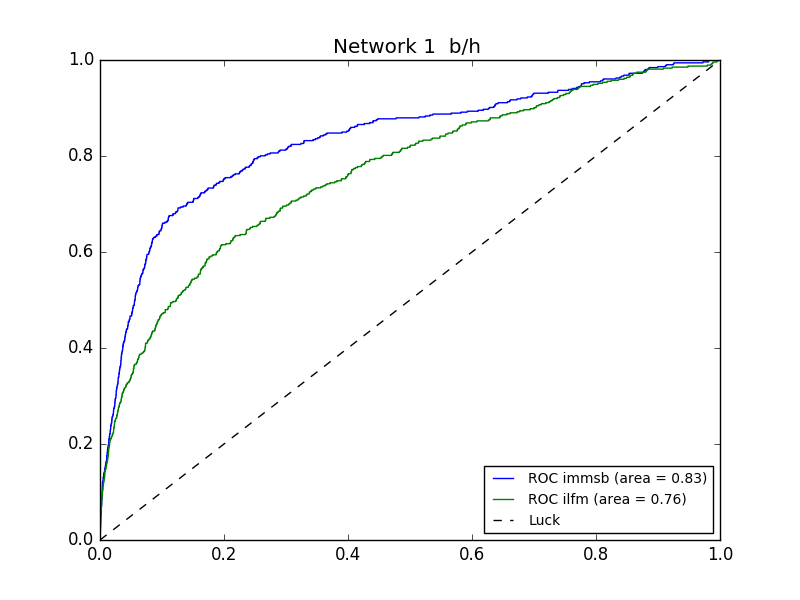
\includegraphics[width=\textwidth]{img/M_e/AUC-ROC/figure_4}
            \label{fig:mean and std of net14}
            \caption {{\small Network1}}    
        \end{subfigure}
        \begin{subfigure}[b]{0.300\textwidth}
            \centering
            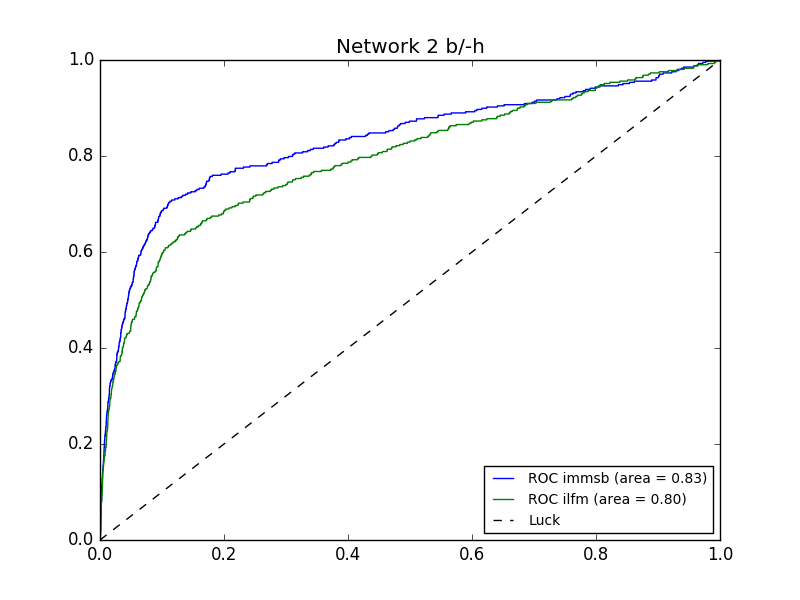
\includegraphics[width=\textwidth]{img/M_e/AUC-ROC/figure_3}
            \label{fig:mean and std of net14}
            \caption {{\small Network2}}    
        \end{subfigure}
        \begin{subfigure}[b]{0.300\textwidth}
            \centering
            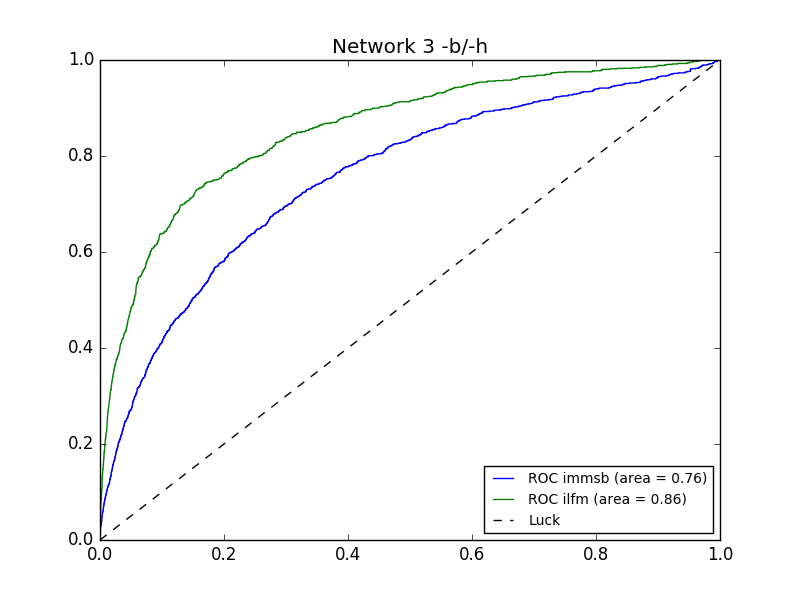
\includegraphics[width=\textwidth]{img/M_e/AUC-ROC/figure_2}
            \label{fig:mean and std of net14}
            \caption {{\small Network3}}    
        \end{subfigure}
        \begin{subfigure}[b]{0.300\textwidth}
            \centering
            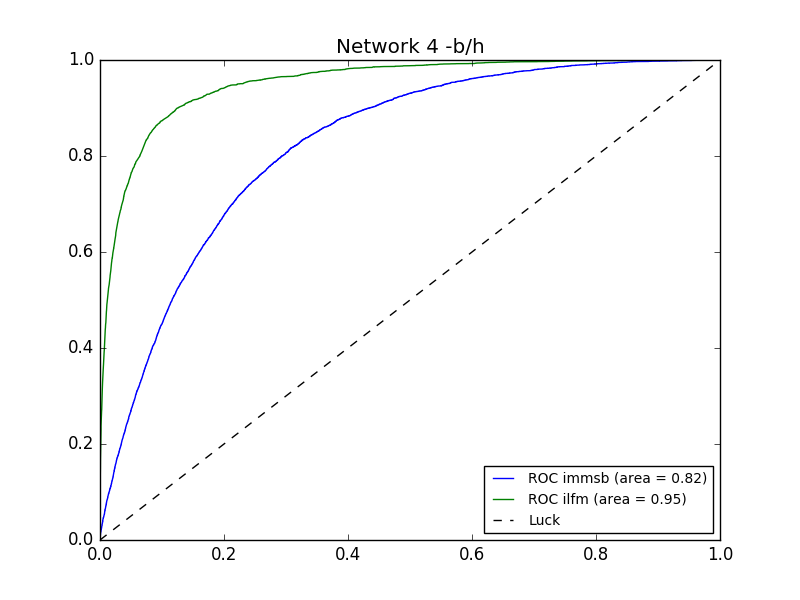
\includegraphics[width=\textwidth]{img/M_e/AUC-ROC/figure_1}
            \label{fig:mean and std of net14}
            \caption {{\small Network4}}    
        \end{subfigure}
        \begin{subfigure}[b]{0.300\textwidth}
            \centering
            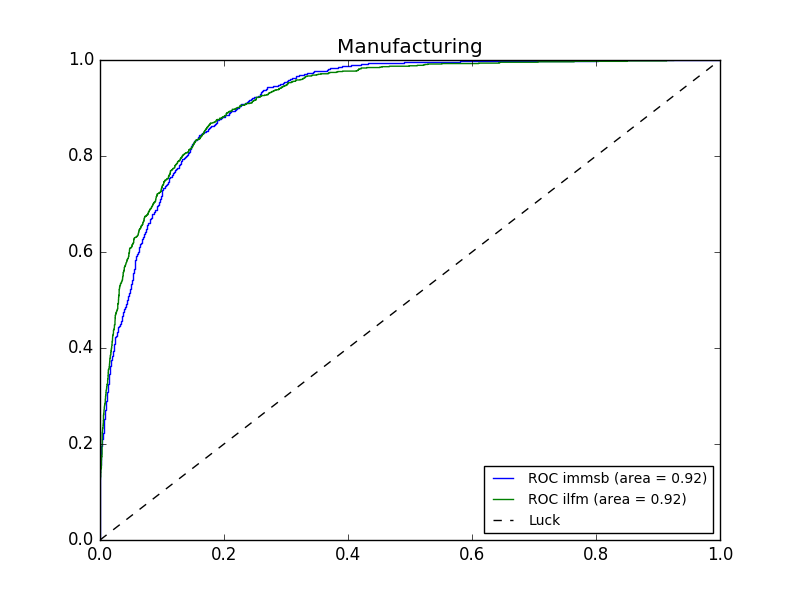
\includegraphics[width=\textwidth]{img/M_e/AUC-ROC/figure_5}
            \label{fig:mean and std of net14}
            \caption {{\small Manufacturing}}    
        \end{subfigure}
        \begin{subfigure}[b]{0.300\textwidth}
            \centering
            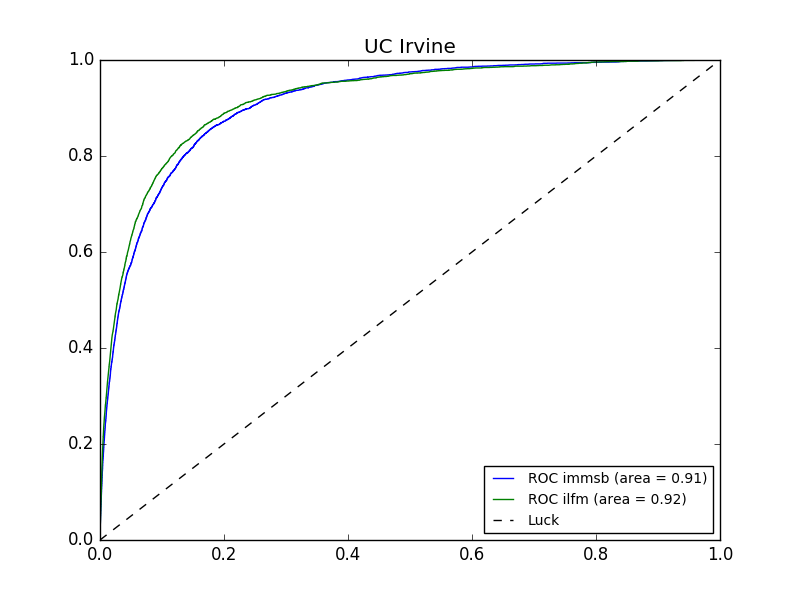
\includegraphics[width=\textwidth]{img/M_e/AUC-ROC/figure_6}
            \caption {{\small UC Irvine}}    
            \label{fig:mean and std of net14}
        \end{subfigure}
        %\quad
        %\hfill
	\caption{AUC curves that compare the performance of ILFM and IMMSB on the 4 synthetic networks.}
	\label{fig:auc}
\end{figure}
